\documentclass[aps, prb, twocolumn, a4paper, floatfix, reprint]{revtex4-2}
\usepackage[%
    margin=10mm,% ако не си принтира 10мм не изглежда грозно, а може да събереш повече текст
    % showframe=true,%
    ]{geometry}
\usepackage[T1,T2A]{fontenc}
\usepackage[utf8]{inputenc}
\usepackage[main=bulgarian, english]{babel}
\usepackage{float}
\AtBeginDocument{\selectlanguage{bulgarian}}
\newcommand{\degree}{^{\circ}}
\usepackage{amsmath}
\usepackage{graphics}
\usepackage{graphicx}
\graphicspath{{.}}
\newcommand{\abs}[1]{\lvert#1\rvert}
\let\phi\varphi
\usepackage{booktabs} % от тук се използва само \midrule може и без него 
%\usepackage{adjustbox} % това може да се използва, за да „смаляваш“ широки таблици
%\usepackage{tabularx} % дефинира колона X в среда tabularx която добавя празно място така че цялата таблица да запълни определена ширина
\usepackage{dcolumn}
\newcolumntype{d}[1]{D{.}{.}{#1}}
\usepackage[unicode=true,pdfusetitle]{hyperref}


\makeatletter
\renewcommand{\Dated@name}{}%
\makeatother



\begin{document}
\title{Теорема на Щайнер}
\author{Васил Николов}
\noaffiliation
\date{03.01.2022}
\maketitle

\section{Цел на упражнението}
Да се изследва торзионно махало, чийто инерчен момент може да се определи, и да се провери теоремата на Щайнер.

\section{Експериментална установка}
Торзионното махало се състои от метален диск с маса $M=99.23g$ с дупки, който е закачен на тънка метална нишка. В дупките могат да се завинтват два малки метални цилиндъра с маса $m=40.6g$. Периодът на махалото зависи от инерчният момент на диска и прикачените за него цилиндри, ако има такива. Така при измерване на периодът на махалото може да се изрази инерчният момент само на цилиндрите, когато са поставени на дадено разстояние от центъра на цилиндъра. 

\section{Теоретична обосновка}
При усукване на нишката на ъгъл $\phi$ на диска се прилага въртящ момент $T = D \phi$, където $D$ е торзионен момент на нишката. Тогава ако инерчният момент на диска е $I$, то периодът на махалото е 
\begin{gather*}
    T = 2\pi \sqrt{\frac{I}{D}} \\
    I = \frac{D}{4 \pi^2}T^2 = kT^2; \ k = \frac{D}{4\pi^2} = const
\end{gather*}
Нека инерчният момент на диска е $I_0$, а инерчният момент на един от цилиндрите спрямо оста му е $I_1$, и нека в общ случай цилиндрите са завинтени в дупка на разстояние $L$ от центъра на диска. Тогава за общия инерчен момент можем да запишем 
\begin{gather*}
    I = I_0 + 2I_1 + 2mL^2\\
    I = kT^2 \\
    \Rightarrow T^2 = \frac{I_0 + 2I_1}{k} + \frac{2m}{k}L^2 \\
\end{gather*}
Ако направим графика на $y=T^2$ и $x=L^2$ очакваме да е права линия, което би доказало теоремата на Щайнер. 

\section{Експериментални данни и резултати}
На Фигура 1 е дадена графика на $y=T^2$ като функция на $x=L^2$. 
\begin{figure}[H]
    \centering
    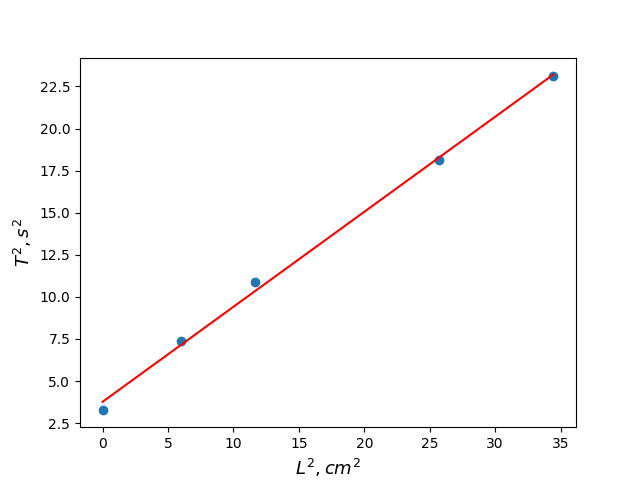
\includegraphics[width=\columnwidth, keepaspectratio=true]{Figure_1.png} 
\end{figure}

Вижда се, че точките много добре се описват от линейна зависимост. Това означава, че данните са в съгласие с теоремата на Щайнер. 

\end{document}